\section{Minimax}
In der Programmierarbeit haben wir mit Java schon zwei Versionen des Minimax-Algorithmus implementiert.
Eine sequentielle (normalfall) und eine parallele (mittels ForkJoin) Lösung.
Da die weiteren Verbesserungen in dieser Arbeit an diesen Implementierungen basieren, werden sie hier kurz Dokumentiert.

\subsection{Minimax sequenziell}
Die sequenzielle Implementierung des Minimax-Algorithmus ist ziemlich unkompliziert.
Es besteht eine rekursive Funktion, die für jeden legalen Schachzug, bis zu einer bestimmten Tiefe, ausgeführt wird.
Die Funktion implementiert die Minimax-Logik mit einer Abweichung vom Standard-Minimax-Algorithmus - sie protokolliert die Zugverläufe für jede Zugkombination.
Dies aus zwei Gründen:
\begin{enumerate}
    \item Erleichtertes Debugging
    \item Bei Zügen mit dem gleichen Ergebnis wird der Zug mit der geringeren Tiefe, bzw.\ kürzeren Historie genommen
\end{enumerate}

Zusätzlich besteht eine vorzeitige Rückgabe bei Zug-Pfaden, welche zum Schluss vom Spiel führen (z.B.\ Schachmatt).
Beispiel: Die angegebene Tiefe ist 5, jedoch wird mit einer Zugkombination nach 3 Zügen Schachmatt erzeugt - somit rechnet die Funktion nur bis zur Tiefe 3.

\begin{figure}[H]
    \centering
    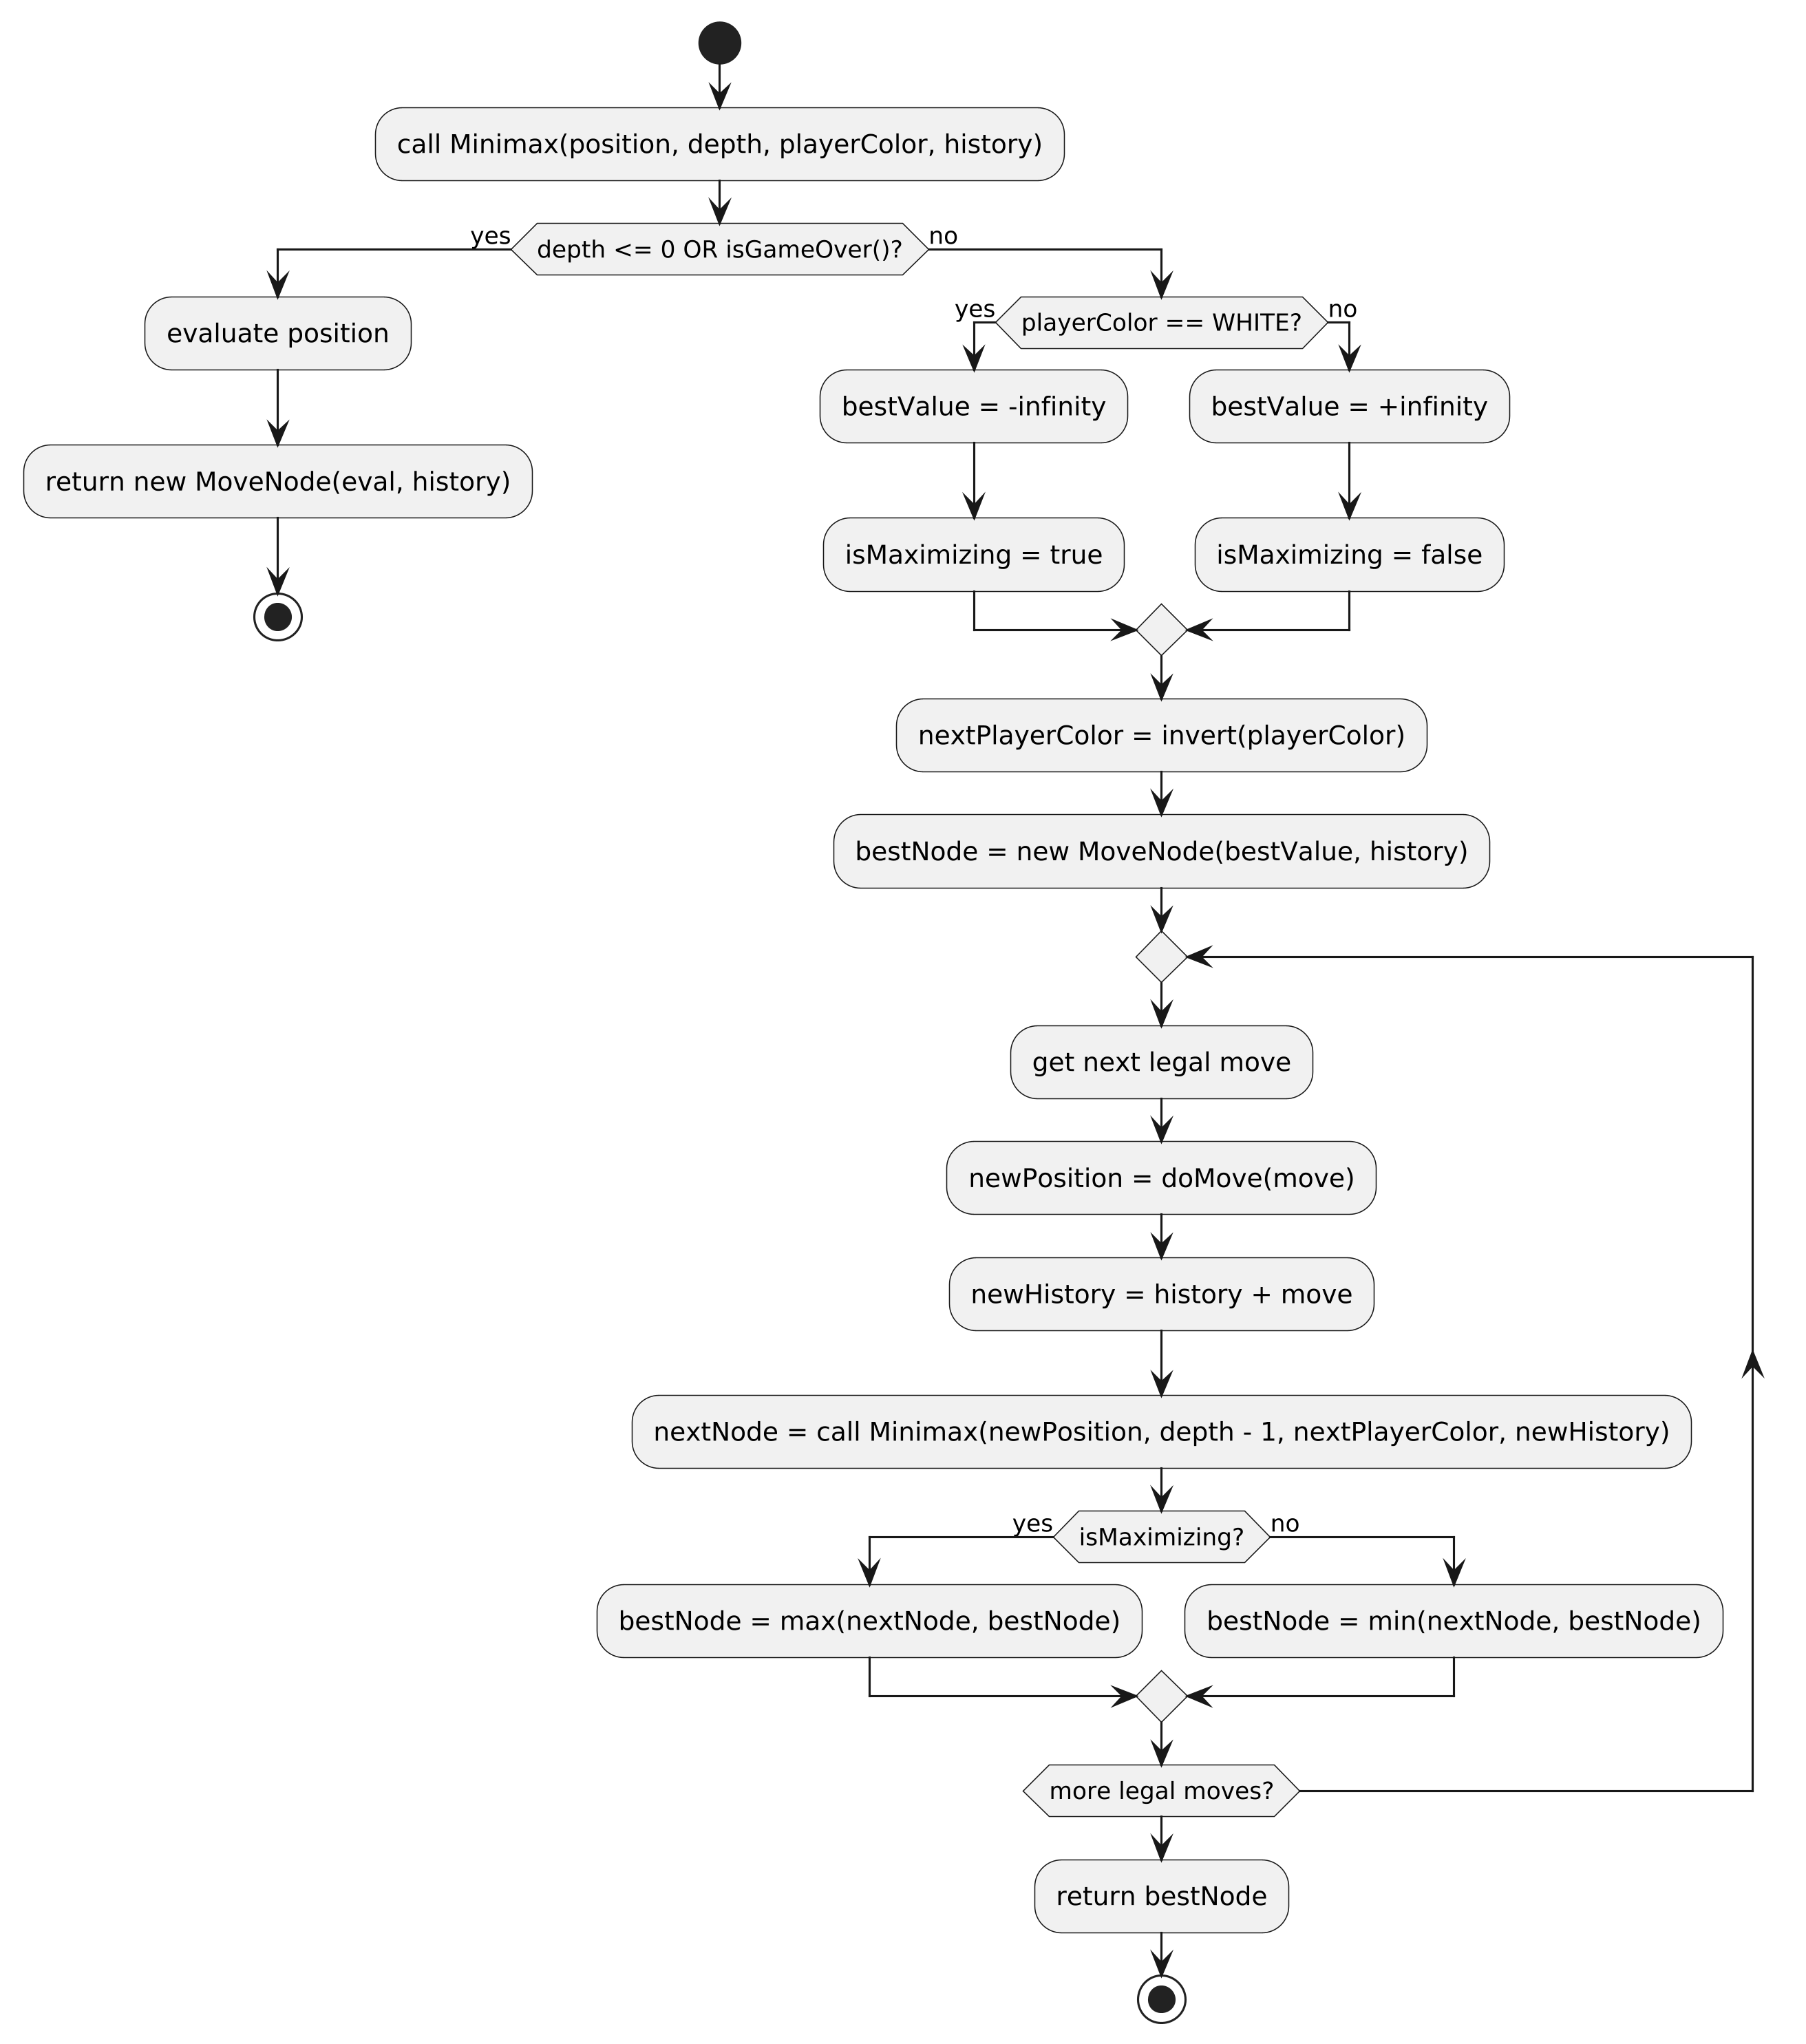
\includegraphics[width=\linewidth]{generated-diagrams/sequential-minimax}
    \caption{Ablaufdiagramm - Minimax sequenziell}
    \label{fig:minimax-sequential}
\end{figure}

\lstinputlisting[
    firstline=26,
    lastline=55,
    firstnumber=26,
    caption={Code - Minimax sequenziell},
    label={lst:minimax-sequenziell}
]{../src/main/java/ch/hslu/cas/msed/blobfish/player/bot/minimax/MiniMaxSequential.java}

\subsection{Minimax parallel}
Die parallele Implementierung enthält die gleiche Basislogik, jedoch wird anstelle einer iteration für alle legale Züge das ForkJoin Prinzip verwendet.
Für jeden legalen Zug wird ein Task erstellt.
Alle erstellten Tasks werden zur Ausführung zum ForkJoin Pool hinzugefügt.
Dies passiert rekursiv für jede Tiefe.
Anschliessend wird gewartet bis alle Tasks einer bestimmten Tiefe fertig sind und die Resultate der Ergebnisse werden durch die Minimax-Logik überprüft.

\begin{figure}[H]
    \centering
    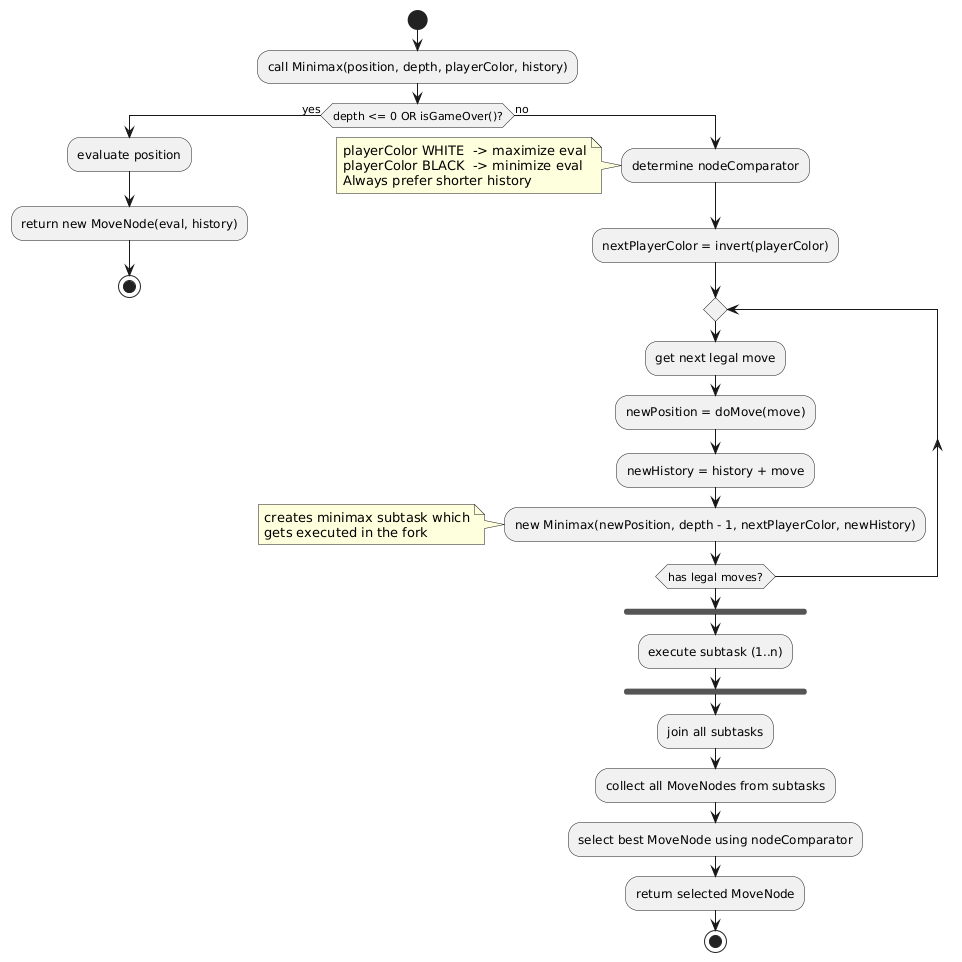
\includegraphics[width=\linewidth]{generated-diagrams/forkjoin-minimax}
    \caption{Ablaufdiagramm - Minimax parallel}
    \label{fig:minimax-parallel}
\end{figure}

\lstinputlisting[
    firstline=12,
    lastline=66,
    firstnumber=12,
    caption={Code - Minimax ForkJoin Task},
    label={lst:minimax-forkjoin-task}
]{../src/main/java/ch/hslu/cas/msed/blobfish/player/bot/minimax/MiniMaxRecursiveTask.java}

\lstinputlisting[
    firstline=15,
    lastline=28,
    firstnumber=15,
    caption={Code - Minimax parallel Task-Aufruf},
    label={lst:minimax-parallel}
]{../src/main/java/ch/hslu/cas/msed/blobfish/player/bot/minimax/MiniMaxParallel.java}


\section{Alpha-Beta-Pruning}
Zunächst war vorgesehen, sämtliche Optimierungen sowohl für die sequenzielle als auch für die parallele Implementierung des Minimax-Algorithmus umzusetzen.
Nach einer Recherche in Alpha-Beta-Pruning ergab sich, dass diese Optimierung für sequentielle Implementierungen vorgesehen ist.

Es bestehen auch Ansätze für parallele Implementierungen, wie Young Brothers Wait Concept.
Die Idee ist, dass der Zug mit der höchsten Wahrscheinlichkeit, der beste zu sein, zuerst evaluiert wird - danach werden alle anderen Züge in parallel evaluiert.
Somit können die restlichen Züge mit dem ersten verglichen werden\ \cite{alphabetaybwc}.

Bei solchen Ansätzen ist jedoch die Umsetzung umständlich und der Leistungsgewinn sehr variabel und unerheblich.
Aus diesen Gründen wurde die Alpha-Beta-Pruning Optimierung nur für die sequenzielle Implementierung umgesetzt.

Die ursprüngliche Implementierung des Minimax-Algorithmus musste nur minim angepasst werden, um diese Optimierung einzubauen.
Es wurden 2 neue Parameter zur Funktion hinzugefügt: alpha und beta.
Diese merken sich die relevanten Werte der vorherigen Evaluationen und anhand dessen wird entschieden, ob die Suche vorzeitig abgebrochen werden kann.
Die relevanten Zeilen sind die Zeilen 63--71.
\lstinputlisting[
    firstline=28,
    lastline=76,
    firstnumber=28,
    caption={Code - Minimax sequenziell mit Alpha-Beta-Pruning},
    label={lst:minimax-sequenziell-alpha-beta}
]{../src/main/java/ch/hslu/cas/msed/blobfish/player/bot/minimax/MiniMaxAlphaBetaSequential.java}

Zusätzlich ist bei dieser Optimierung die Reihenfolge der Züge wichtig.
Darum werden sie auf den Zeilen 42--43 sortiert.
Die Sortierung ist erstmals sehr primitiv - es werden Züge, die eine Figur fangen, zuerst ausgewertet, da diese eine grössere Chance haben bessere Werte zu liefern.
Mit dem Einbau weiterer Heuristiken wird auch diese Sortierung erweitert.